\documentclass[10pt,a4paper]{article}
\usepackage[T1]{fontenc}
\usepackage[a4paper]{geometry}
\usepackage{xcolor}
\usepackage{amssymb}
\usepackage{amsmath}
\usepackage{graphicx}
\usepackage{tabularx}
\usepackage{multirow}
\usepackage{subfigure}
\usepackage{verbatim}
\usepackage{fancyhdr}
\usepackage{listings}
\usepackage{../common/espacs}

%\input{../common/commands.tex}

\title{Exercise Session 4}
\date{October 26, 2012}

\pagestyle{fancy}
\headheight 35pt

\rhead{\copyright~2006/2012}

\newcommand{\vv}[1]{\mathbf{#1}}

\begin{document}
\lstset{language=[ISO]C++}
\maketitle

\section*{Google PageRank}

Google has become the most used search engine in a very small amount of time
after its creation. This success depends on the accuracy of the results that
was highly better than the other search engines. Google generates its own
\emph{ranking} of the importance of the web pages in order to sort the results
of a query. This ranking is what the user is interested in.

The algorithm that sorts web pages based on their importance is called
\emph{PageRank} and it has been developed by S.~Brin and L.~Page at Stanford
University \cite{Brin1998}. The basic principle is as follows
\begin{itemize}

    \item if a web page A has a \emph{link} to a page B, this is interpreted as
    a vote by A in favour of B, so B's place in the ranking is raised;

    \item the voters are not all the same: the vote from someone who is high in
    the ranking (someone who has many votes) weights more than someone who is
    low-ranked.

\end{itemize}

\begin{figure}
    \centering
    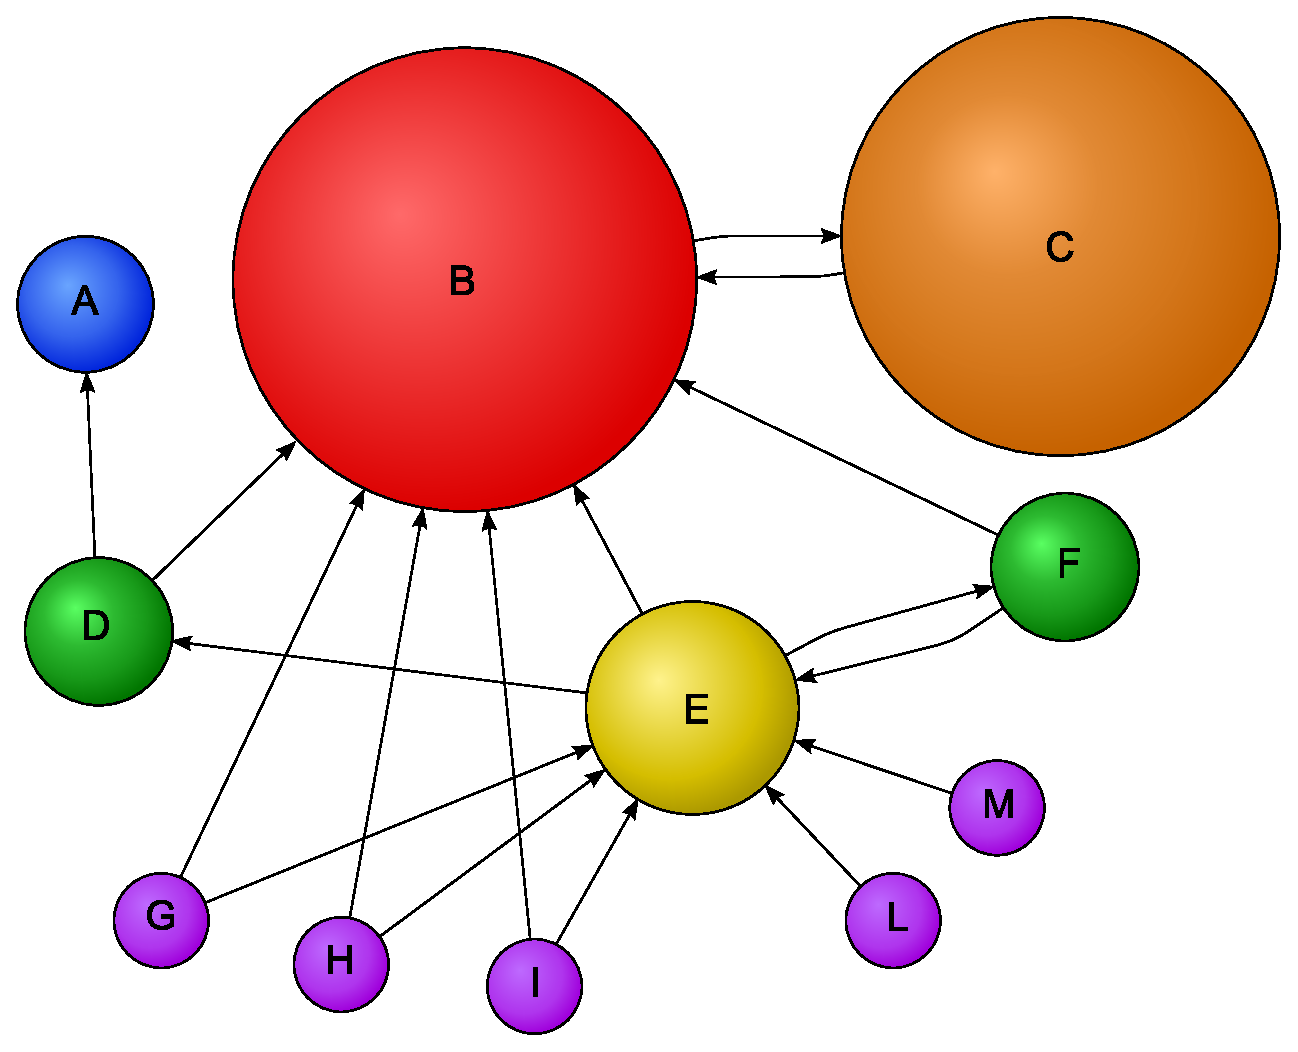
\includegraphics[width=0.6\textwidth]{./fig/PageRanks_Example_only_letters}
    \caption{Schematic diagram of the \emph{ranking}: every sphere represents
    a web page, every arrow a link. The dimension of the sphere measures the
    importance of the page.}
    \label{fig:PR}
\end{figure}

This principle is depicted in Fig.~\ref{fig:PR}. Page B receives many links and
therefore it is considered very important. Page C is more important than page E,
even if it has less links, since a vote from B matters more than many small
links that E gets (i.e. if the \emph{Washington Post} or the
\emph{New York Times} would publish a link to the website for the PACS course,
this link would count more than the links coming from the personal page of the
professor, his assistant and the students of the course!).

In a more formal way, the \emph{ranking} $r(p)$ of the page $p$ is defined as
the sum of all the \emph{rankings} $r(q)$ of all the pages $q$ that link to $p$
\begin{align}
    \label{eq:rank}
    r(p)=\sum_{q \rightarrow p} \frac{r(q)}{\#q}
\end{align}
The sum is weighted with $\#q$, the number of links in the page $q$ (if the page
$q$ has only one link towards $p$ it is likely that an interested reader would
follow it, on the other hand, if the page $q$ has many links, it is less likely
that the reader would choose the link to $p$).
It is simple to notice that this is an implicit problem: in order to compute the
ranking of $p$ we need the ranking of the other pages, that are in turn based on
the ranking of $p$.

The problem is simplified by writing it in a matricial form. Let $\{p_1, p_2,
\dots, p_N\}$ be all the pages and $A \in \mathbb{R}^{N \times N}$ be the
connection matrix, with $a_{i,j}$ given by
\begin{align}
      \label{eq:harmonicp}
      a_{i,j}=
      \begin{cases}
        \dfrac{1}{\#p_j} & \text{if there is a link from $p_j$ to $p_i$} \\[1ex]
        0 &  \mbox{otherwise}
      \end{cases}
\end{align}
Note that the $a_{i,j}$ can be interpreted as a probability distribution, in
particular they decsribe the probability that a person who clicks randomly
walks from the page $p_j$ to the page $p_i$. The matrix $A$ has the following
property
\begin{align} \label{eq:sum1}
    \sum_{i=1}^{N} a_{i,j}=1
\end{align}

If the ranking of the pages $p_i$ is represented by the column vector $\vv{r} =
[r_1, r2, \dots, r_N]^T$, called \emph{PageRank}, \eqref{eq:rank} is equivalent
to
\begin{align*}
    \vv{r}=A \vv{r}
\end{align*}
Therefore, the \emph{PageRank} is the eigenvector that corresponds to the
eigenvalue $1$ of the associated eigenvalue problem. It can be demonstrated
that, if the $\lambda_i$ are the eigenvalues of $A$, then $|\lambda_i| \leq 1$.
Moreover, $\lambda_1=1$ has molteplicity one\footnote{A sufficient condition is
given by the Perron Frobenius theorem, that requires a matrix that corresponds
to an irriducible graph. A trick to satisfy the hypothesis could be to assign
a link to every existing page without links.}.

Since the number $N$ of analyzed pages is in the order of the tens of billions,
the computation of the \emph{PageRank} eigenvector with a direct method is
computationally expensive, even for the ones that have extraordinary
computational resources. We therefore use an iterative method, that gives an
approximate solution: the power method. In this particular case, stopping the
iterations at the step $k$ means that we consider only the pages $p_j$ that
are $k$ clicks away from $p_i$\footnote{For semplicity reasons we disregard the
possibility to introduce a \emph{damping fatctor} \cite{Brin1998}, that does
not modify the basic principle of the algorithm.}.

\subsection*{Power method}

The \emph{power method} can be applied to matrices in which the maximum modulus
eigenvalue $\lambda_1$ has molteplicity one and it is well separated from the
closest eigenvalue with a smaller modulus. Here follows the generic step $k$ of
the algorithm
\begin{align*}
    {\bf q}\iter{k} &= \frac{ A{\bf q}\iter{k-1} }{
        \norm{ A{\bf q}\iter{k-1}}_2 } \\
    {\bf \nu}\iter{k} &= {{\bf q}\iter{k}}^T  A {\bf q}\iter{k} \\
    {\bf w}\iter{k} &= \frac{ {{\bf w}\iter{k-1}}^T A }{
        \norm{ {{\bf w}\iter{k-1}}^T A}_2 }
\end{align*}
where $\nu\iter{k}$, ${\bf q}\iter{k}$ and ${\bf w}\iter{k}$ are the
approximation of $\lambda_1$ and the aproximations of the left and right
eigenvector ${\bf x}_1$ e ${\bf y}_1$ associated to it. The following estimate
holds
\begin{align*}
    \module{ \lambda_1 - \nu\iter{k} } \approx %
    \frac{ \norm{ {\bf r}\iter{k} }_2 }{
    \module{ {{\bf w}\iter{k}}^T \cdot{\bf q}\iter{k} } }
\end{align*}
where ${\bf r}\iter{k} \eqbydef A{\bf q}\iter{k} - \nu\iter{k}{\bf
q}\iter{k}$ is the residual at iteration $k$. The estimate can be used to
implement a convergence criterion.

\subsection*{Linear algebra library: Eigen}

In order to solve the eigenvalue problem we need a linear algebra library. In
this course we adopt the \texttt{Eigen} library version 3.1, that can manage
dense and sparse matrices.


\section*{Esercizio 1}

Starting from the example \texttt{QuadratureRule/baseVersion}
\begin{enumerate}
  \item extend the use of GetPot in order to pass the integrand function
  directly from the data file

  \item add a Gaussian quadrature rule, templatized on the number of quadrature
  points. The Gaussian rule should derive from the common base class
  \cpp{StandardQuadratureRule}. The points and weights can be computed using the
  \texttt{legendre\_rule} library

  \item compute the integral of the function
    \begin{align*}
    f(x) = e^x x
    \end{align*}
  in $[0,1]$ using all the available quadrature rules.

  \item implement a MonteCarlo quadrature rule, that also derives from
  \cpp{QuadratureRule}.
\end{enumerate}


\subsection*{Exercise 1 solution}

The solution for the exercise is as follows
%
\lstset{basicstyle=\scriptsize\sf}
    \lstinputlisting{./src/all_in_one/bn-allinone.cpp}
\lstset{basicstyle=\sf}

First of all, we have defined a user type called \cpp{real}. If we want to
change the precision for the calculations, it will be sufficient to just change
the definition for the \cpp{real} type. All the code would be updated
coherently.

In order to have the possibility to pass an arbitrary function to the method
that performs the evaluation of the zero we use a \emph{function pointer}. The
instruction
\begin{lstlisting}
typedef real (*fctptr)(real);
\end{lstlisting}
defines a type \cpp{fctptr} as a pointer to a function that have a \cpp{real} as
argument and thta have a \cpp{real} as return value.

we can adopt different strategies to stop the iterations of a method that
computes a zero. When the function derivative absolute value is close to $1$ in
the neighborhood of the zero an efficient way to set a stop criterion is by
using the \emph{residual}. More specifically, we consider that the method as
converged at the iteration $k$ when $\module{\function{f}{x\iter{k}}} <
\cpp{tol}$.

An alternative way, based on a check on the \emph{increment}, is instead
suitable for fixed point iterations when the derivative of the iteration
function $\function{\phi}{\cdot}$ is far away from $1$ in modulus near the zero.
The criterion stops the iterations when $\module{x\iter{k+1} - x\iter{k}} <
\cpp{tol}$. For the Newton's method, where $\function{\phi'}{\alpha} = 0$ by
definition, the check on the increment is a typical choice. The implementation
takes care of the different types of stop criteria with an \emph{enumeration},
called \cpp{checkT}. Every method has a member \cpp{M\_check} of type
\cpp{checkT} that chooses the convergence criterion.

If we compile with
\begin{verbatim}
    g++ -o bn-allinone bn-allinone.cpp -Wall
\end{verbatim}
and execute the resulting program we get
\begin{verbatim}
0.707107        27
0.707107        7
0.707107        14 1
\end{verbatim}



\bibliographystyle{siam}
%\bibliography{../common/bibliography}

\begin{thebibliography}{9}

\bibitem{Brin1998} S.~Brin and L.~Page,
The anatomy of a large-scale hypertextual web search engine,
{\em Computer Networks and ISDN Systems}, vol.~30, no.~1-7, pp.~107 -- 117,
1998. Proceedings of the Seventh International World Wide Web Conference.

\end{thebibliography}

\end{document}
